\section{溶液物性および圧力場の確認}
\subsection{粘度計測}
鋼球落下実験を行う試験溶液として,1wt.\%PAA溶液の製作を行った.この製作した溶液の粘度特性を確認し,先行研究\cite{ref:9}\cite{ref:10}における粘度特性と比較した.この比較を行うことで先行研究との粘度特性の違いを確認した.なお,この粘度計測を実施するためには,溶質が溶媒に十分に均一に溶解することならびに,混合時に混入した気泡がおおむね消失することが必要であるため,溶液製作1週間後に行った.それぞれの試料に対し,円錐回転子の回転数を変化させ,各5回計測を行いその平均を求めた.

水道水の粘度計測を行った結果をFig.\ref{fig:water-vis}に示す.なお,縦軸は粘度,横軸はせん断速度を表す.2.2においても示したが,コーンロータの回転速度を変化させることにより,せん断速度を変化させた.その結果,粘度は約1.1[mPa$\cdot$ s]でほぼ一定となっていた.これは,水がニュートン流体であり,粘度を比例係数とした速度勾配とせん断応力の比例関係となっているためであると考えられる.

水道水の場合と同様にPAA溶液の粘度計測を行った結果をFig.\ref{fig:PAA-vis}に示す.なお,縦軸は粘度の対数,横軸はせん断速度の対数を表す.また,Iwamuro {\it et al.}\cite{ref:9}やShiratori {\it et al.}\cite{ref:10}の文献値も共に示した.ここで,粘度$\mu$はせん断速度$\dot{\gamma}$に対して,粘度定数 k[Pa$\cdot$ $\text{s}^n$],指数$n$を用い Power-law modelに従うものとすると,
\begin{eqnarray}
    \label{eq:power-low}
    \mu=k\cdot\dot{\gamma}^{n-1}
\end{eqnarray}
といった式で与えられる\cite{ref:1}.式\ref{eq:power-low}を用いて近似線計算を行った結果を,Table\ref{table:power-law}に示す.今回作製したPAA溶液の粘度特性はIwamuro {\it et al.}とShiratori {\it et al.}の間に位置しており,適切に作製されたと判断できる.

\begin{figure}[ht]
    \centering
    \includegraphics[width=12cm,clip]{4-Results/water.png}
    \caption{Meansured viscosity versus shear rate for tap water.}
    \label{fig:water-vis}
\end{figure}

\begin{figure}[ht]
    \centering
    \includegraphics[width=13cm,clip]{4-Results/PAA-viscosity.png}
    \caption{Flow curve for 1wt.\%PAA solution.}
    \label{fig:PAA-vis}
\end{figure}

\begin{table}[h]
    \centering
    \caption{}
    \label{table:power-law}
    \begin{tabular}{c|c|c} \hline
        & k & n \\ \hline \hline
        Present Value & 8.37 & 0.24 \\
        Iwamuro\cite{ref:8} & 9.4 & 0.23 \\
        Shiratori \textit{et al}.(2016)\cite{ref:10} & 5.9 & 0.25 \\ \hline
    \end{tabular}
\end{table}

\newpage

\subsection{圧力場 計測結果}

容器Aにおける超音波圧力場の計測を行った結果をFig.\ref{fig:pressure}(a),容器Bにおける超音波圧力場の計測を行った結果をFig.\ref{fig:pressure}(b)に示す.縦軸は水槽底面からの高さ,横軸は圧力である.この結果を元にTable\ref{table:press-A},\ref{table:press-B} に圧力$P$の$y$方向平均値を示す.どちらの水槽においても水槽全体に圧力場が形成されていることが分かった.また,先行研究であるIwamuro \textit{et al}.\cite{ref:8},\cite{ref:9}と同様な圧力平均値となった.

\begin{table}[h]
    \centering
    \caption{Averaged value of pressure data in tank A.}
    \label{table:press-A}
    \begin{tabular}{c|c|c}\hline
                       & Present 1wt.\% PAA & Iwamuro {\it et al.}\cite{ref:8} \\ \hline
        $\bar{P}$[kPa] &       68        & 72                              \\ \hline
    \end{tabular}
\end{table}

\begin{table}[h]
    \centering
    \caption{Averaged value of pressure data in tank B.}
    \label{table:press-B}
    \begin{tabular}{c|c|c}\hline
                       & Present 1wt.\% PAA & Iwamuro \cite{ref:9} \\ \hline
        $\bar{P}$[kPa] & 159.2              & 180                              \\ \hline
    \end{tabular}
\end{table}

\begin{figure}[ht]
    \centering
    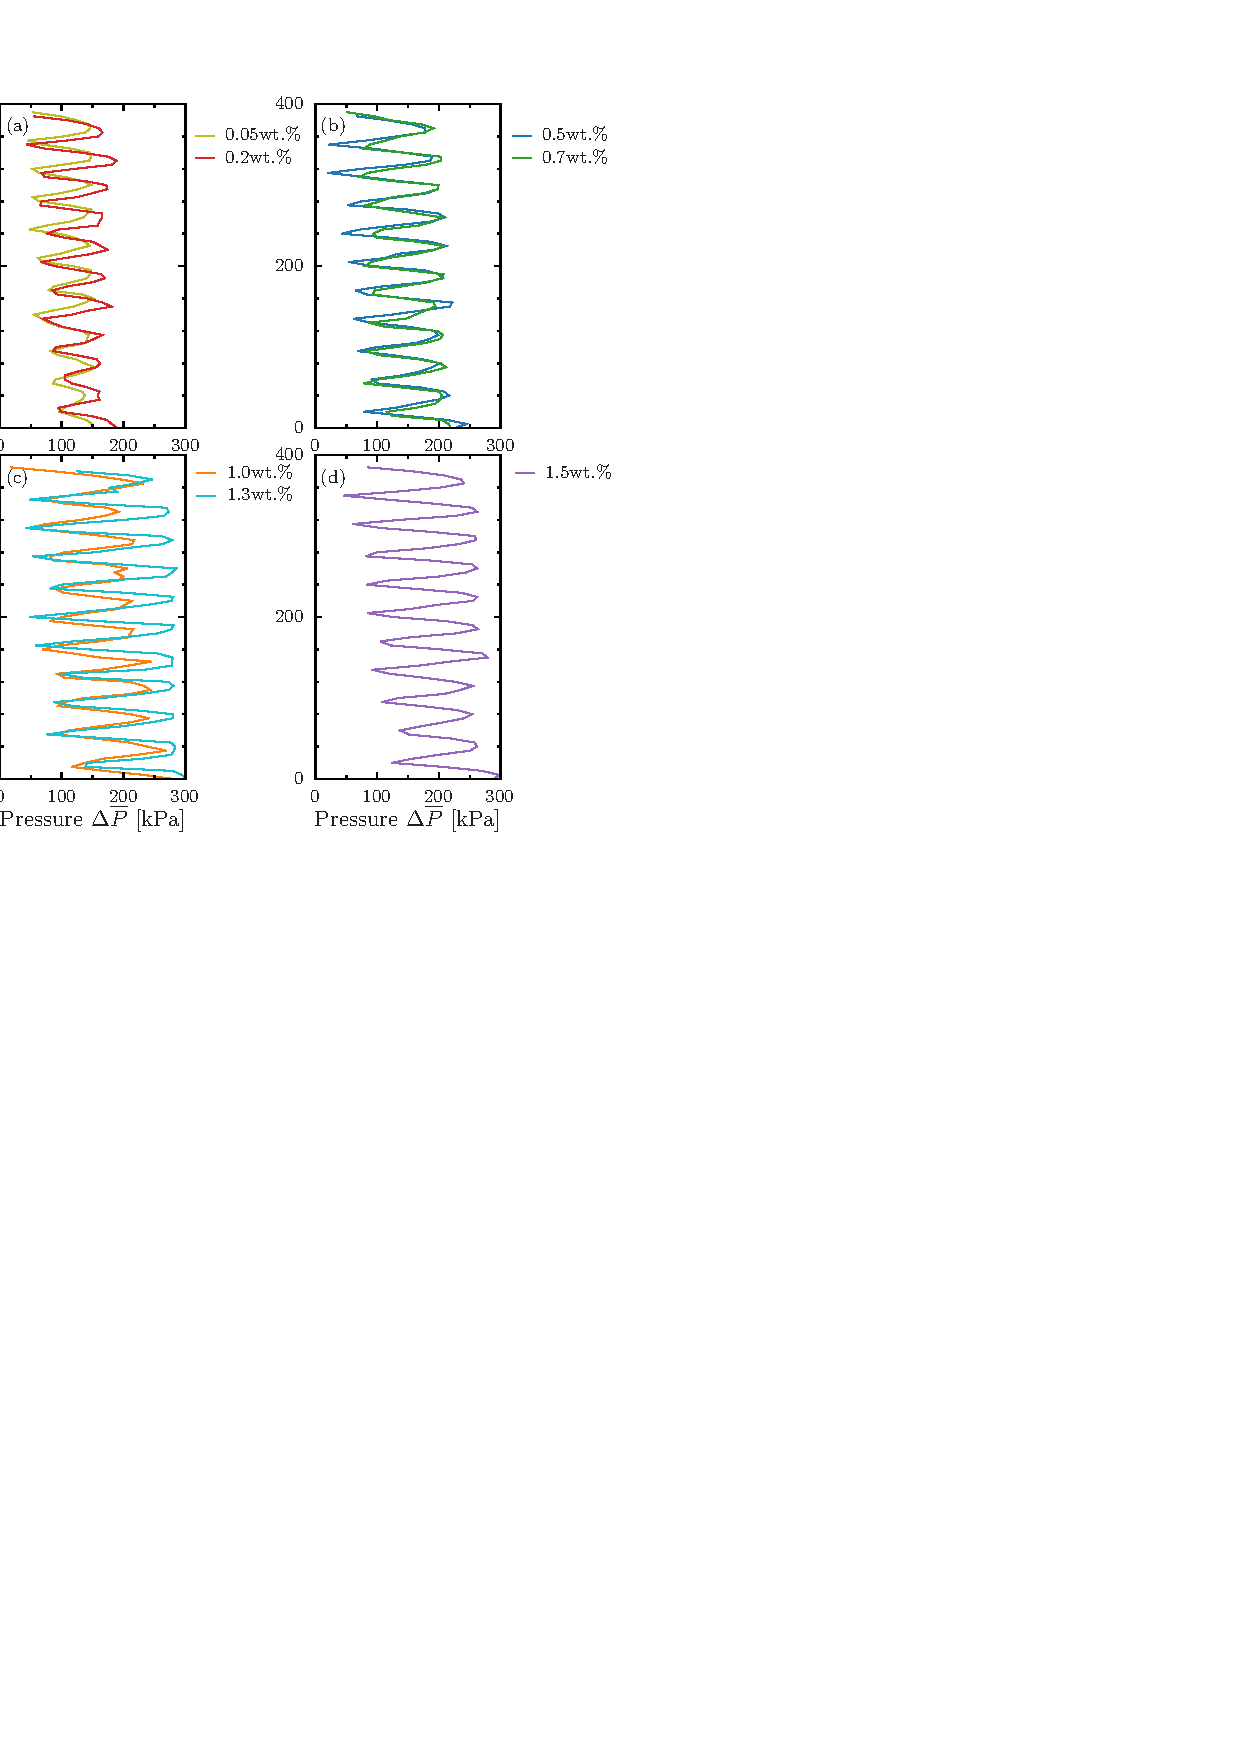
\includegraphics[width=12cm,clip]{4-Results/press.png}
    \caption{Pressure field in PAA solution measurement results. (a)In tank A. (b)In tank B.}
    \label{fig:pressure}
\end{figure}
